% answers.tex —— 2003 年·全国旧课程卷·文科 · 参考答案与详细解析片段
% 由 tools/generate_projects.py 依来源总账自 2003/2003_数学真题_全国旧课程文_试题.md + 2003/2003_数学真题_全国旧课程文_解析正文.md + 2003/2003_数学真题_全国旧课程文_答案要点.md 生成，勿手改（改源 MD 后重跑）


\begin{gktip}
固定源 PDF 为印刷页码 136–137 的两页题面，不附答案。以下解析均依据题面独立复算；第 16、17、21、22 题图形在 LaTeX 工程中以 TikZ/PGFPlots 矢量源重绘。
\end{gktip}

\gkpart{一、选择题}

\begin{answer}
\gksolhead{1}{}

\textbf{题目}：

直线 $y=2x$ 关于 $x$ 轴对称的直线方程为\mbox{（　　）}

（A）$y=-\dfrac12x$　　（B）$y=\dfrac12x$　　（C）$y=-2x$　　（D）$y=2x$

\Needspace{4\baselineskip}
\textbf{解析}

关于 $x$ 轴对称把点 $(x,y)$ 变为 $(x,-y)$，故 $y=2x$ 变为 $y=-2x$，选 C。

\gkanswer{答案：C}

\end{answer}
\begin{answer}
\gksolhead{2}{}

\textbf{题目}：

已知 $x\in\left(-\dfrac\pi2,0\right)$，$\cos x=\dfrac45$，则 $\tan2x=$\mbox{（　　）}

（A）$\dfrac7{24}$　　（B）$-\dfrac7{24}$　　（C）$\dfrac{24}{7}$　　（D）$-\dfrac{24}{7}$

\Needspace{4\baselineskip}
\textbf{解析}

\Needspace{5\baselineskip}
由 $x\in(-\pi/2,0)$ 得 $\sin x=-3/5$、$\tan x=-3/4$。因此

\nopagebreak[4]
\[
\tan2x=\frac{2\tan x}{1-\tan^2x}
=\frac{-3/2}{7/16}=-\frac{24}{7},
\]

选 D。

\gkanswer{答案：D}

\end{answer}
\begin{answer}
\gksolhead{3}{}

\textbf{题目}：

抛物线 $y=ax^2$ 的准线方程是 $y=2$，则 $a$ 的值为\mbox{（　　）}

（A）$\dfrac18$　　（B）$-\dfrac18$　　（C）$8$　　（D）$-8$

\Needspace{4\baselineskip}
\textbf{解析}

写成 $x^2=\dfrac1a y$，抛物线的准线为 $y=-\dfrac1{4a}$。由 $-\dfrac1{4a}=2$ 得 $a=-1/8$，选 B。

\gkanswer{答案：B}

\end{answer}
\begin{answer}
\gksolhead{4}{}

\textbf{题目}：

等差数列 $\{a_n\}$ 中，已知 $a_1=\dfrac13$，$a_2+a_5=4$，$a_n=33$，则 $n$ 为\mbox{（　　）}

（A）48　　（B）49　　（C）50　　（D）51

\Needspace{4\baselineskip}
\textbf{解析}

\Needspace{5\baselineskip}
设公差为 $d$，则

\nopagebreak[4]
\[
a_2+a_5=\frac23+5d=4,\qquad d=\frac23.
\]

于是 $a_n=\dfrac13+\dfrac23(n-1)=\dfrac{2n-1}{3}$。令其等于 $33$，得 $n=50$，选 C。

\gkanswer{答案：C}

\end{answer}
\begin{answer}
\gksolhead{5}{}

\textbf{题目}：

双曲线虚轴的一个端点为 $M$，两个焦点为 $F_1\text{、}F_2$，$\angle F_1MF_2=120^\circ$，则双曲线的离心率为\mbox{（　　）}

（A）$\sqrt3$　　（B）$\dfrac{\sqrt6}{2}$　　（C）$\dfrac{\sqrt6}{3}$　　（D）$\dfrac{\sqrt3}{3}$

\Needspace{4\baselineskip}
\textbf{解析}

\Needspace{5\baselineskip}
设双曲线实、虚半轴为 $a_0\text{、}b$，焦半距为 $c$。在直角三角形 $F_1MF_2$ 的等腰三角形中，

\nopagebreak[4]
\[
\cos120^\circ
=\frac{MF_1^2+MF_2^2-F_1F_2^2}{2MF_1MF_2}
=1-\frac{2c^2}{a_0^2+2b^2}.
\]

\Needspace{5\baselineskip}
得 $a_0^2=2b^2$，所以 $c^2=a_0^2+b^2=\dfrac32a_0^2$，离心率为

\nopagebreak[4]
\[
e=\frac ca=\frac{\sqrt6}{2}.
\]

选 B。

\gkanswer{答案：B}

\end{answer}
\begin{answer}
\gksolhead{6}{}

\textbf{题目}：

\Needspace{5\baselineskip}
设函数

\nopagebreak[4]
\[
f(x)=
\begin{cases}
2^{-x}-1,&x\leqslant0,\\
x^2,&x>0,
\end{cases}
\]

若 $f(x_0)>1$，则 $x_0$ 的取值范围是\mbox{（　　）}

（A）$(-1,1)$　　（B）$(-1,+\infty)$

（C）$(-\infty,-2)\cup(0,+\infty)$　　（D）$(-\infty,-1)\cup(1,+\infty)$

\Needspace{4\baselineskip}
\textbf{解析}

当 $x\leqslant0$ 时，$2^{-x}-1>1$ 等价于 $x<-1$；当 $x>0$ 时，$x^2>1$ 等价于 $x>1$。故选 D。

\gkanswer{答案：D}

\end{answer}
\begin{answer}
\gksolhead{7}{}

\textbf{题目}：

已知 $f(x^5)=\lg x$，则 $f(2)=$\mbox{（　　）}

（A）$\lg2$　　（B）$\lg32$　　（C）$\lg\dfrac1{32}$　　（D）$\dfrac15\lg2$

\Needspace{4\baselineskip}
\textbf{解析}

\Needspace{5\baselineskip}
令 $x^5=2$，即 $x=2^{1/5}$，代入 $f(x^5)=\lg x$ 得

\nopagebreak[4]
\[
f(2)=\lg 2^{1/5}=\frac15\lg2.
\]

选 D。

\gkanswer{答案：D}

\end{answer}
\begin{answer}
\gksolhead{8}{}

\textbf{题目}：

函数 $y=\sin(x+\varphi)$（$0\leqslant\varphi\leqslant\pi$）是 $\mathbb R$ 上的偶函数，则 $\varphi=$\mbox{（　　）}

（A）$0$　　（B）$\dfrac\pi4$　　（C）$\dfrac\pi2$　　（D）$\pi$

\Needspace{4\baselineskip}
\textbf{解析}

\nopagebreak[4]
\[
\sin(x+\varphi)=\sin x\cos\varphi+\cos x\sin\varphi.
\]

要成为偶函数，必须 $\cos\varphi=0$。结合 $0\leqslant\varphi\leqslant\pi$ 得 $\varphi=\pi/2$，选 C。

\gkanswer{答案：C}

\end{answer}
\begin{answer}
\gksolhead{9}{}

\textbf{题目}：

已知点 $(a,2)$（$a>0$）到直线 $l:x-y+3=0$ 的距离为 $1$，则 $a=$\mbox{（　　）}

（A）$\sqrt2$　　（B）$2-\sqrt2$　　（C）$\sqrt2-1$　　（D）$\sqrt2+1$

\Needspace{4\baselineskip}
\textbf{解析}

\Needspace{5\baselineskip}
点到直线的距离给出

\nopagebreak[4]
\[
\frac{|a-2+3|}{\sqrt2}=1
\Longrightarrow |a+1|=\sqrt2.
\]

因 $a>0$，所以 $a=\sqrt2-1$，选 C。

\gkanswer{答案：C}

\end{answer}
\begin{answer}
\gksolhead{10}{}

\textbf{题目}：

已知圆锥的底面半径为 $R$、高为 $3R$，它的内接圆柱的底面半径为 $\dfrac34R$，该圆柱的全面积为\mbox{（　　）}

（A）$2\pi R^2$　　（B）$\dfrac94\pi R^2$　　（C）$\dfrac83\pi R^2$　　（D）$\dfrac52\pi R^2$

\Needspace{4\baselineskip}
\textbf{解析}

\Needspace{5\baselineskip}
设圆柱高为 $h$。由圆锥截面相似，

\nopagebreak[4]
\[
h=3R\left(1-\frac{3}{4}\right)=\frac{3R}{4}.
\]

\Needspace{5\baselineskip}
圆柱全面积为

\nopagebreak[4]
\[
2\pi\left(\frac{3R}{4}\right)^2
+2\pi\frac{3R}{4}\frac{3R}{4}
=\frac94\pi R^2,
\]

选 B。

\gkanswer{答案：B}

\end{answer}
\begin{answer}
\gksolhead{11}{}

\textbf{题目}：

已知长方形的四个顶点 $A(0,0)\text{、}B(2,0)\text{、}C(2,1)\text{、}D(0,1)$，一质点从 $AB$ 的中点 $P_0$ 沿与 $AB$ 的夹角为 $\theta$ 的方向射到 $BC$ 上的点 $P_1$ 后，依次反射到 $CD\text{、}DA$ 和 $AB$ 上的点 $P_2\text{、}P_3$ 和 $P_4$（入射角等于反射角）。若 $P_4$ 与 $P_0$ 重合，则 $\tan\theta=$\mbox{（　　）}

（A）$\dfrac13$　　（B）$\dfrac25$　　（C）$\dfrac12$　　（D）$1$

\Needspace{4\baselineskip}
\textbf{解析}

\Needspace{5\baselineskip}
把矩形边界展开，若反射光线最终回到 $P_0$，展开后的直线经过相应的中点；由对称性，$P_1\text{、}P_2\text{、}P_3$ 均为相应边的中点。第一段从 $P_0(1,0)$ 到 $P_1(2,1/2)$，故

\nopagebreak[4]
\[
\tan\theta=\frac{1/2}{1}=\frac12.
\]

选 A。

\gkanswer{答案：C}

\end{answer}
\begin{answer}
\gksolhead{12}{}

\textbf{题目}：

一个四面体的所有棱长都为 $\sqrt2$，四个顶点在同一球面上，则此球的表面积为\mbox{（　　）}

（A）$3\pi$　　（B）$4\pi$　　（C）$3\sqrt3\pi$　　（D）$6\pi$

\Needspace{4\baselineskip}
\textbf{解析}

\Needspace{5\baselineskip}
正四面体棱长为 $\sqrt2$，外接球半径为

\nopagebreak[4]
\[
R=\frac{\sqrt6}{4}\cdot\sqrt2=\frac{\sqrt3}{2}.
\]

所以球面面积为 $4\pi R^2=3\pi$，选 A。

\gkanswer{答案：A}

\end{answer}
\gkpart{二、填空题}

\begin{answer}
\gksolhead{13}{}

\textbf{题目}：

不等式 $\sqrt{4x-x^2}<x$ 的解集是\gkblank{}。

\Needspace{4\baselineskip}
\textbf{解析}

\Needspace{5\baselineskip}
定义域要求 $0\leqslant x\leqslant4$，且右侧要求 $x>0$。平方得

\nopagebreak[4]
\[
4x-x^2<x^2
\Longleftrightarrow x>2.
\]

故解集为 $(2,4]$。

\gkanswer{答案：$(2,4]$}

\end{answer}
\begin{answer}
\gksolhead{14}{}

\textbf{题目}：

$\left(x^2-\dfrac1{2x}\right)^9$ 的展开式中 $x^9$ 的系数是\gkblank{}。

\Needspace{4\baselineskip}
\textbf{解析}

\Needspace{5\baselineskip}
通项为

\nopagebreak[4]
\[
\binom9k(x^2)^{9-k}\left(-\frac1{2x}\right)^k,
\]

\Needspace{5\baselineskip}
幂次为 $18-3k$。令 $18-3k=9$ 得 $k=3$，所求系数为

\nopagebreak[4]
\[
\binom93\left(-\frac12\right)^3=-\frac{21}{2}.
\]

\gkanswer{答案：$-\dfrac{21}{2}$}

\end{answer}
\begin{answer}
\gksolhead{15}{}

\textbf{题目}：

在平面几何里，有勾股定理：“设 $\triangle ABC$ 的两边 $AB\text{、}AC$ 互相垂直，则 $AB^2+AC^2=BC^2$。”拓展到空间，类比平面几何的勾股定理，研究三棱锥的侧面面积与底面面积间的关系，可以得出的正确结论是：“设三棱锥 $A-BCD$ 的三个侧面 $ABC\text{、}ACD\text{、}ADB$ 两两互相垂直，则\gkblank{}。”

\Needspace{4\baselineskip}
\textbf{解析}

\Needspace{5\baselineskip}
设三条互相垂直的棱长为 $u,v,w$，则三个侧面面积分别为 $uv/2\text{、}vw/2\text{、}wu/2$，底面为三边向量构成的三角形。直接用向量叉积或海伦公式化简，得

\nopagebreak[4]
\[
S_{BCD}^2=S_{ABC}^2+S_{ACD}^2+S_{ADB}^2.
\]

\gkanswer{答案：$S_{BCD}^2=S_{ABC}^2+S_{ACD}^2+S_{ADB}^2$}

\end{answer}
\begin{answer}
\gksolhead{16}{}

\textbf{题目}：

如图，一个地区分为 5 个行政区域，现给地图着色，要求相邻地区不得使用同一颜色，现有 4 种颜色可供选择，则不同的着色方法共有\gkblank{}种。（以数字作答）
\nopagebreak[4]
\begin{center}% 2003 年全国旧课程文科第 16 题：行政区域着色图
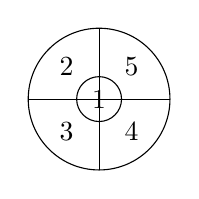
\begin{tikzpicture}[scale=0.75]
  \draw (0,0) circle (1.2);
  \draw (0,-1.2)--(0,1.2) (-1.2,0)--(1.2,0);
  \draw (0,0) circle (0.38);
  \node at (0,0) {1};
  \node at (-0.55,0.55) {2};
  \node at (0.55,0.55) {5};
  \node at (-0.55,-0.55) {3};
  \node at (0.55,-0.55) {4};
\end{tikzpicture}
\end{center}
\nopagebreak[4]
\Needspace{4\baselineskip}
\textbf{解析}

\Needspace{5\baselineskip}
中央区域必须先选颜色，有 $4$ 种；外围四个区域构成一个四边形环，使用剩余三种颜色且相邻不同，着色数为

\nopagebreak[4]
\[
(3-1)^4+(3-1)=18.
\]

总数为 $4\times18=72$。

\gkanswer{答案：$72$}

\end{answer}
\gkpart{三、解答题}

\begin{answer}
\gksolhead{17}{}

\textbf{题目}：

已知正四棱柱 $ABCD-A_1B_1C_1D_1$，$AB=1$，$AA_1=2$，$E$ 为 $CC_1$ 中点，$F$ 为 $BD_1$ 中点。
\nopagebreak[4]
\begin{center}% 2003 年全国旧课程文科第 17 题：正四棱柱
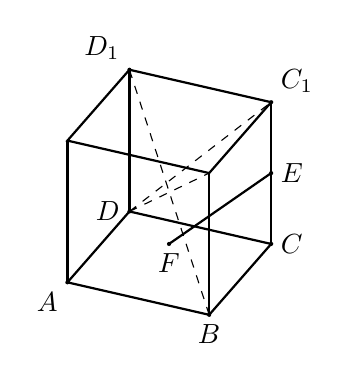
\begin{tikzpicture}[>=stealth,scale=0.75]
  \coordinate (A) at (0,0); \coordinate (B) at (2.4,-0.55);
  \coordinate (C) at (3.45,0.65); \coordinate (D) at (1.05,1.2);
  \coordinate (A1) at (0,2.4); \coordinate (B1) at (2.4,1.85);
  \coordinate (C1) at (3.45,3.05); \coordinate (D1) at (1.05,3.6);
  \coordinate (E) at (3.45,1.85); \coordinate (F) at (1.72,0.65);
  \draw[thick] (A)--(B)--(C)--(D)--cycle;
  \draw[thick] (A1)--(B1)--(C1)--(D1)--cycle;
  \draw[thick] (A)--(A1) (B)--(B1) (C)--(C1) (D)--(D1);
  \draw[dashed] (B)--(D1) (D)--(B1) (D)--(C1);
  \draw[thick] (E)--(F);
  \fill (A) circle (1pt) node[below left] {$A$};
  \fill (B) circle (1pt) node[below] {$B$};
  \fill (C) circle (1pt) node[right] {$C$};
  \fill (D) circle (1pt) node[left] {$D$};
  \fill (D1) circle (1pt) node[above left] {$D_1$};
  \fill (C1) circle (1pt) node[above right] {$C_1$};
  \fill (E) circle (1pt) node[right] {$E$};
  \fill (F) circle (1pt) node[below] {$F$};
\end{tikzpicture}
\end{center}
\nopagebreak[4]
（1） 证明：$EF$ 为 $BD_1$ 与 $CC_1$ 的公垂线；

（2） 求点 $D_1$ 到面 $BDE$ 的距离。

\Needspace{4\baselineskip}
\textbf{解析}

\Needspace{5\baselineskip}
取

\nopagebreak[4]
\[
A=(0,0,0),\ B=(1,0,0),\ C=(1,1,0),\ D=(0,1,0),
\]

\nopagebreak[4]
\[
A_1=(0,0,2),\ B_1=(1,0,2),\ C_1=(1,1,2),\ D_1=(0,1,2).
\]

此时 $E=(1,1,1)$、$F=(1/2,1/2,1)$。

\gksubpart{(1)}

\Needspace{5\baselineskip}
有

\nopagebreak[4]
\[
\overrightarrow{EF}=\left(-\frac12,-\frac12,0\right),\quad
\overrightarrow{BD_1}=(-1,1,2),\quad
\overrightarrow{CC_1}=(0,0,2).
\]

因此 $\overrightarrow{EF}$ 同时垂直于 $BD_1$ 和 $CC_1$，且 $EF$ 分别与两线相交于 $F\text{、}E$，所以 $EF$ 是两异面直线的公垂线。

\gksubpart{(2)}

\Needspace{5\baselineskip}
平面 $BDE$ 的一个法向量为

\nopagebreak[4]
\[
(\overrightarrow{BD}\times\overrightarrow{BE})=(1,1,-1),
\]

\Needspace{5\baselineskip}
其方程为 $x+y-z-1=0$。故

\nopagebreak[4]
\[
d(D_1,\text{\text{平面} }BDE)
=\frac{|0+1-2-1|}{\sqrt3}
=\frac2{\sqrt3}.
\]

\gkanswer{答案（1）：见解析版。}

\gkanswer{答案（2）：$\dfrac{2}{\sqrt3}$。}

\end{answer}
\begin{answer}
\gksolhead{18}{}

\textbf{题目}：

已知复数 $z$ 的辐角为 $60^\circ$，且 $|z-1|$ 是 $|z|$ 和 $|z-2|$ 的等比中项，求 $|z|$。

\Needspace{4\baselineskip}
\textbf{解析}

\Needspace{5\baselineskip}
令 $z=re^{i\pi/3}$。由等比中项条件，

\nopagebreak[4]
\[
|z-1|^2=|z|\,|z-2|.
\]

\Needspace{5\baselineskip}
两边平方并利用

\nopagebreak[4]
\[
|z-1|^2=r^2-r+1,\qquad |z-2|^2=r^2-2r+4,
\]

\Needspace{5\baselineskip}
得

\nopagebreak[4]
\[
(r^2-r+1)^2=r^2(r^2-2r+4)
\Longrightarrow r^2+2r-1=0.
\]

因 $r>0$，故 $|z|=r=\sqrt2-1$。

\gkanswer{答案：$|z|=\sqrt2-1$}

\end{answer}
\begin{answer}
\gksolhead{19}{}

\textbf{题目}：

已知数列 $\{a_n\}$ 满足 $a_1=1$，$a_n=3^{n-1}+a_{n-1}$（$n\geqslant2$）。

（1） 求 $a_2\text{、}a_3$；

（2） 证明：$a_n=\dfrac{3^n-1}{2}$。

\Needspace{4\baselineskip}
\textbf{解析}

\gksubpart{(1)}

\Needspace{5\baselineskip}
由递推式

\nopagebreak[4]
\[
a_2=3+1=4,\qquad a_3=9+4=13.
\]

\Needspace{5\baselineskip}
用归纳法可得

\nopagebreak[4]
\[
a_n=1+3+\cdots+3^{n-1}=\frac{3^n-1}{2}.
\]

\gksubpart{(2)}

该等比数列求和式即为所需通项，归纳验证完成证明。

\gkanswer{答案（1）：$a_2=4,\ a_3=13$。}

\gkanswer{答案（2）：$a_n=\dfrac{3^n-1}{2}$。}

\end{answer}
\begin{answer}
\gksolhead{20}{}

\textbf{题目}：

\Needspace{5\baselineskip}
已知函数

\nopagebreak[4]
\[
f(x)=2\sin x(\sin x+\cos x).
\]

（1） 求函数 $f(x)$ 的最小正周期和最大值；

（2） 在给出的直角坐标系中，画出函数 $y=f(x)$ 在区间 $\left[-\dfrac\pi2,\dfrac\pi2\right]$ 上的图象。
\nopagebreak[4]
\begin{center}% 2003 年全国旧课程文科第 20 题：函数图象坐标系
\begin{tikzpicture}[x=1.0cm,y=0.7cm,>=stealth]
  \draw[->] (-1.9,0)--(1.9,0) node[right] {$x$};
  \draw[->] (0,-1.4)--(0,1.6) node[above] {$y$};
  \node[below] at (-1.57,0) {$-\frac\pi2$};
  \node[below] at (1.57,0) {$\frac\pi2$};
  \node[below left] at (0,0) {$O$};
\end{tikzpicture}
\end{center}
\nopagebreak[4]
\Needspace{4\baselineskip}
\textbf{解析}

\gksubpart{(1)}

\Needspace{5\baselineskip}
先化简

\nopagebreak[4]
\[
f(x)=2\sin x(\sin x+\cos x)
=1-\cos2x+\sin2x
=1+\sqrt2\sin\left(2x-\frac\pi4\right).
\]

因此最小正周期为 $\pi$，最大值为 $1+\sqrt2$。

\gksubpart{(2)}

\Needspace{5\baselineskip}
在 $\left[-\pi/2,\pi/2\right]$ 上取关键点

\nopagebreak[4]
\[
\left(-\frac\pi2,1\right),\quad
\left(-\frac\pi4,0\right),\quad
(0,1),\quad
\left(\frac\pi4,2\right),\quad
\left(\frac\pi2,1\right),
\]

按函数曲线平滑连接即可。

\gkanswer{答案（1）：最小正周期为 $\pi$，最大值为 $1+\sqrt2$。}

\gkanswer{答案（2）：见解析版。}

\end{answer}
\begin{answer}
\gksolhead{21}{}

\textbf{题目}：

在某海滨城市附近海面有一台风。据监测，当前台风中心位于城市 $O$（如图）的东偏南 $\theta$ 方向 300 km 的海面 $P$ 处，并以 20 km/h 的速度向西偏北 $45^\circ$ 方向移动，台风侵袭的范围为圆形区域，当前半径为 60 km，并以 10 km/h 的速度不断增大，问几小时后该城市开始受到台风的侵袭？
\nopagebreak[4]
\begin{center}% 2003 年全国旧课程文科第 21 题：台风运动示意图
\begin{tikzpicture}[>=stealth,scale=0.72]
  \draw[->] (-2.8,0)--(3.2,0) node[right] {东};
  \draw[->] (0,-2.3)--(0,2.5) node[above] {北};
  \fill (0,0) circle (1.5pt) node[below left] {$O$};
  \fill (-1.8,-1.25) circle (1.5pt) node[below] {$P$};
  \draw[->,thick] (-1.8,-1.25)--(0.2,0.75) node[midway,below] {$20$ km/h};
  \draw[dashed] (-1.8,-1.25) circle (0.55);
  \node at (-1.35,-1.75) {$r(t)$};
  \draw[->] (0.35,0.1) arc[start angle=15,end angle=210,radius=0.35];
\end{tikzpicture}
\end{center}
\nopagebreak[4]
\Needspace{4\baselineskip}
\textbf{解析}

\Needspace{5\baselineskip}
取 $O$ 为原点，正东方向为 $x$ 轴。题设给出 $OP=300$ km、$\cos\theta=\sqrt2/10$；台风中心以 $20$ km/h 向西偏北 $45^\circ$ 移动，半径为 $60+10t$。把台风中心的坐标代入

\nopagebreak[4]
\[
OP(t)=60+10t
\]

并平方化简，取最早正根，得到 $t=12$。所以 12 小时后城市开始受到台风侵袭。

\gkanswer{答案：12 小时。}

\end{answer}
\begin{answer}
\gksolhead{22}{}

\textbf{题目}：

\Needspace{5\baselineskip}
已知常数 $a>0$，在矩形 $ABCD$ 中，$AB=4$，$BC=4a$，$O$ 为 $AB$ 的中点，点 $E\text{、}F\text{、}G$ 分别在 $BC\text{、}CD\text{、}DA$ 上移动，且

\nopagebreak[4]
\[
\frac{BE}{BC}=\frac{CF}{CD}=\frac{DG}{DA},
\]

$P$ 为 $GE$ 与 $OF$ 的交点（如图）。问是否存在两个定点，使 $P$ 到这两点的距离之和为定值？若存在，求出这两点的坐标及此定值；若不存在，请说明理由。
\nopagebreak[4]
\begin{center}% 2003 年全国旧课程文科第 22 题：矩形动点示意图
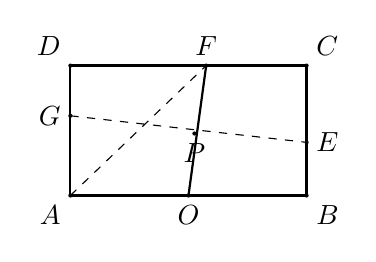
\begin{tikzpicture}[>=stealth,scale=0.75]
  \coordinate (A) at (0,0); \coordinate (B) at (4,0);
  \coordinate (C) at (4,2.2); \coordinate (D) at (0,2.2);
  \coordinate (E) at (4,0.9); \coordinate (F) at (2.3,2.2);
  \coordinate (G) at (0,1.35); \coordinate (P) at (2.1,1.05);
  \coordinate (O) at (2,0);
  \draw[thick] (A)--(B)--(C)--(D)--cycle;
  \draw[dashed] (G)--(E) (A)--(F);
  \draw[thick] (O)--(F);
  \fill (A) circle (1pt) node[below left] {$A$};
  \fill (B) circle (1pt) node[below right] {$B$};
  \fill (C) circle (1pt) node[above right] {$C$};
  \fill (D) circle (1pt) node[above left] {$D$};
  \fill (E) circle (1pt) node[right] {$E$};
  \fill (F) circle (1pt) node[above] {$F$};
  \fill (G) circle (1pt) node[left] {$G$};
  \fill (P) circle (1pt) node[below] {$P$};
  \fill (O) circle (1pt) node[below] {$O$};
\end{tikzpicture}
\end{center}
\nopagebreak[4]
\Needspace{4\baselineskip}
\textbf{解析}

\Needspace{5\baselineskip}
设

\nopagebreak[4]
\[
\frac{BE}{BC}=\frac{CF}{CD}=\frac{DG}{DA}=k,
\qquad 0\leqslant k\leqslant1.
\]

\Needspace{5\baselineskip}
建立坐标系

\nopagebreak[4]
\[
A=(-2,0),\ B=(2,0),\ C=(2,4a),\ D=(-2,4a),\ O=(0,0).
\]

\Needspace{5\baselineskip}
则

\nopagebreak[4]
\[
E=(2,4ak),\quad F=(2-4k,4a),\quad G=(-2,4a-4ak).
\]

\Needspace{5\baselineskip}
令 $t=2k-1$，联立直线 $GE$ 与 $OF$ 得

\nopagebreak[4]
\[
x=-\frac{2t}{t^2+2},\qquad y=\frac{4a}{t^2+2}.
\]

\Needspace{5\baselineskip}
消去 $t$：

\nopagebreak[4]
\[
2a^2x^2+(y-a)^2=a^2.
\]

\Needspace{5\baselineskip}
这是以 $(0,a)$ 为中心的椭圆弧。若 $0<a<1/\sqrt2$，焦点为

\nopagebreak[4]
\[
\left(\pm\sqrt{\frac12-a^2},a\right),
\qquad |PE|+|PF|=\sqrt2;
\]

\Needspace{5\baselineskip}
若 $a>1/\sqrt2$，焦点为

\nopagebreak[4]
\[
\left(0,a\pm\sqrt{a^2-\frac12}\right),
\qquad |PE|+|PF|=2a.
\]

当 $a=1/\sqrt2$ 时为圆，取中心为重合焦点，距离和为 $\sqrt2$。

\gkanswer{答案：当 $0<a<\dfrac1{\sqrt2}$ 时，取焦点 $\left(\pm\sqrt{\dfrac12-a^2},a\right)$，距离和为 $\sqrt2$；当 $a=\dfrac1{\sqrt2}$ 时为圆，取中心为重合焦点，距离和为 $\sqrt2$；当 $a>\dfrac1{\sqrt2}$ 时，取焦点 $\left(0,a\pm\sqrt{a^2-\dfrac12}\right)$，距离和为 $2a$。}

\end{answer}